\documentclass{article}
\usepackage[dvipdfmx]{graphicx}
\usepackage{fancyvrb}
\usepackage{amsmath}
\setlength{\textheight}{22cm}
\setlength{\textwidth}{17cm}
\setlength{\leftmargin}{-1 in}
\setlength{\topmargin}{0.35in}
\setlength{\topmargin}{0.1in}
\setlength{\evensidemargin}{0. in}
\setlength{\oddsidemargin}{0. in}

\newenvironment{code}
{
 \VerbatimEnvironment
 \begin{Verbatim}[frame=single]%
}
{
 \end{Verbatim}%
}

\begin{document}


\parindent 0pt
\parskip 5 pt
\title{Sunway TaihuLight Programming By examples}
\author{The Codesign Team, RIKEN AICS}
\maketitle
\thispagestyle{empty}

\begin{abstract}
  Sunway TaihuLight is the supercomputer with the largest peak performance on the Earth
  at the moment.
  We would like to understand what kind of application can be executed on TaihuLight,
  what are the theoretical limits of the performance of those applications,
  and how the actual implementations achieve closer to the theoretically-given performance limits.

  The architecture of Sunway TaihuLight is different from those of
  modern computers.  Many of modern computers have multi-level memory
  hierarchy, such as: the L1, L2, L3 cache, and the main memory. On
  the contrary, Sunway TaihuLight has only two levels of memory: the
  local directive memory (LDM) is the only memory layer above the main
  memory. The core group (CG) consists of 64 computing processor
  element (CPEs) organized in 8x8 mesh.

  These architectures pose unique challenge in the optimization on
  Sunway TaihuLight. On the other hand, they provide high performance
  if we are able to understand the architectures and use them in the
  right way.

  Therefore, we summarize the knowledge for using the Sunway TaihuLight in this document,
  by collecting the set of source codes
  for Sunway TaihuLight
  and their execution and benchmark results.


\end{abstract}

\newpage\tableofcontents\newpage

\section{Exercises} \label{sec:exercises}

\subsection{Introduction to the exercises section}


% 練習編では、Sunway TaihuLightのプログラミングに必要なプリミティブを順次取り上げ、実際に動くプログラムを作りながら動作を確認していく。
In \S \ref{sec:exercises} we practice and confirm the various programming primitives of Sunway TaihuLight
by working examples.

\subsection{Hello World}
\subsubsection{Introduction}

One of the most simple way of programming Sunway TaihuLight is to use only the
MPE
(Management Processing Element).
The MPE can be programmed in vanilla C/C++. Let us first write some program
that run on MPE.




\subsubsection{Source code}
 We have compiled and executed the following source codes:

\verb`master.c`
\begin{code}
#include <stdio.h>
#include <athread.h>
#include <fcntl.h>
#define N 4096


//extern SLAVE_FUN(func)();

double a[N];
double b[N];
double c[N];

int main() {
  int i;
  printf("hello Sunway TaihuLight\n");

  for (i=0; i<N;++i){
    a[i] = i;
    b[i] = i;
  }

  for (i=0; i<N;++i){
    c[i] = a[i] * b[i];
  }

  for (i=1; i<N; i=2*i+1){
    printf("%d^2 == %lf\n", i, c[i]);
  }

  return 0;
}

\end{code}

\verb`run.sh`
\begin{code}

cd /home/export/base/nsccwuxi_riken/riken/online1/sandbox/nushio_box/sunway-test/01-master/src/
make && make run
    
\end{code}

\subsubsection{Results}

Got the following results:

\begin{code}
# 2017-02-15 00:20:49.556760
$ chmod 755 /home/nushio/hub/GB17/sunway-test/01-master/src/run.sh
$ ssh sunway 'mkdir -p /home/export/base/nsccwuxi_riken/riken/online1/sandbox/nushio_box/sunway-test/01-master/src/'
$ rsync -avz /home/nushio/hub/GB17/sunway-test/01-master/src/ sunway:/home/export/base/nsccwuxi_riken/riken/online1/sandbox/nushio_box/sunway-test/01-master/src/
sending incremental file list
./
Makefile
run.sh

sent 436 bytes  received 72 bytes  145.14 bytes/sec
total size is 955  speedup is 1.88
$ ssh sunway /home/export/base/nsccwuxi_riken/riken/online1/sandbox/nushio_box/sunway-test/01-master/src//run.sh
make: `all' に対して行うべき事はありません.
bsub -I -b -q q_sw_expr -n 1 -cgsp 64 -share_size 4096 -host_stack 128 ./main.out
Job <6419562> has been submitted to queue <q_sw_expr>
waiting for dispatch ...
hello Sunway TaihuLight
1^2 == 1.000000
3^2 == 9.000000
7^2 == 49.000000
15^2 == 225.000000
31^2 == 961.000000
63^2 == 3969.000000
127^2 == 16129.000000
255^2 == 65025.000000
511^2 == 261121.000000
1023^2 == 1046529.000000
2047^2 == 4190209.000000
4095^2 == 16769025.000000
dispatching ...
Job 6419562 has been finished.

\end{code}

\subsubsection{Discussion}

We have programmed MPE.


\subsection{The use of the CPE}
\subsubsection{Introduction}

The most of the computational power of Sunway TaihuLight resides in the
CPE(Computing Processing Element)s in the
CG(core group)s.


The MPE programs and the CPE programs must be compiled with
the \verb`-host` flag and
the \verb`-slave` flag, respectively.

A
\verb`-hybrid`
flag is required when linking.

We use the following syntax
to declare a
CPE function in the
MPE program:


\begin{code}
extern SLAVE_FUN(func)();
\end{code}

And call it via
\verb`athread_spawn`

\begin{code}
athread_spawn(func,0);
athread_join();
\end{code}

The second argument, \verb`void *arg` of the
\verb`athread_spawn` is the functional argument to \verb`func`.


Use \verb`athread_get` and \verb`athread_put` to communicate data between the MPE and the CPE.





\subsubsection{Source code}
 We have compiled and executed the following source codes:

\verb`master.c`
\begin{code}
#include <stdlib.h>
#include <stdio.h>
#include <athread.h>
#include <sys/types.h>
#include <sys/stat.h>
#include <fcntl.h>

#define N 4096


extern SLAVE_FUN(func)();

double a[N];
double b[N];
double c[N];

int main() {
  int i;
  printf("hello Sunway TaihuLight\n");

  for (i=0; i<N;++i){
    a[i] = i;
    b[i] = i;
  }

  // for (i=0; i<N;++i){
  //   c[i] = a[i] * b[i];
  // }
  athread_init();
  athread_spawn(func,0);//fflush(NULL);
  athread_join();

  for (i=1; i<N; i=2*i+1){
    printf("%d^2 == %lf\n", i, c[i]);
  }
  athread_halt();
  return 0;
}

\end{code}

\verb`slave.c`
\begin{code}
#include <slave.h>
#include <math.h>
#include <dma.h>

#define N 4096
#define I 64

__thread_local volatile unsigned long get_reply, put_reply;
__thread_local int my_id;
__thread_local double a_slave[I], b_slave[I], c_slave[I];
extern double a[N], b[N], c[N];

void func() {
  int i;
  my_id = athread_get_id(-1);
  get_reply = 0;

  athread_get(PE_MODE, &a[my_id*I], &a_slave[0],I*8,&get_reply,0,0,0);
  athread_get(PE_MODE, &b[my_id*I], &b_slave[0],I*8,&get_reply,0,0,0);
  while(get_reply!=2) {}

  for(i=0;i<I;i++){
    c_slave[i]=a_slave[i]*b_slave[i];
  }

  put_reply=0;
  athread_put(PE_MODE,&c_slave[0],&c[my_id * I],I*8,&put_reply,0,0);
  while(put_reply!=1) {}

}

\end{code}

\verb`run.sh`
\begin{code}

cd /home/export/base/nsccwuxi_riken/riken/online1/sandbox/nushio_box/sunway-test/02-slave/src/
make && make run
    
\end{code}

\subsubsection{Results}

Got the following results:

\begin{code}
# 2017-02-14 20:29:33.736609
$ chmod 755 /home/nushio/hub/GB17/sunway-test/02-slave/src/run.sh
$ ssh sunway 'mkdir -p /home/export/base/nsccwuxi_riken/riken/online1/sandbox/nushio_box/sunway-test/02-slave/src/'
$ rsync -avz /home/nushio/hub/GB17/sunway-test/02-slave/src/ sunway:/home/export/base/nsccwuxi_riken/riken/online1/sandbox/nushio_box/sunway-test/02-slave/src/
sending incremental file list
./
Makefile
master.c
run.sh
slave.c

sent 1,298 bytes  received 98 bytes  146.95 bytes/sec
total size is 1,995  speedup is 1.43
$ ssh sunway /home/export/base/nsccwuxi_riken/riken/online1/sandbox/nushio_box/sunway-test/02-slave/src//run.sh
sw5cc.new -O3 -msimd -host -E master.c > master.e
#	sw5cc.new -O3 -msimd -host -s master.c -o master.s
sw5cc.new -O3 -msimd -host -c master.c -o master.o
sw5cc.new -O3 -msimd -slave -E slave.c > slave.e
#sw5cc.new -O3 -msimd -slave -s slave.c -o slave.s
sw5cc.new -O3 -msimd -slave -c slave.c -o slave.o
sw5cc.new -hybrid  master.o slave.o -o main.out
bsub -I -b -q q_sw_expr -n 1 -cgsp 64 -share_size 4096 -host_stack 128 ./main.out
Job <6419252> has been submitted to queue <q_sw_expr>
some node is sleeping, waiting for dispatch ...
hello Sunway TaihuLight
1^2 == 1.000000
3^2 == 9.000000
7^2 == 49.000000
15^2 == 225.000000
31^2 == 961.000000
63^2 == 3969.000000
127^2 == 16129.000000
255^2 == 65025.000000
511^2 == 261121.000000
1023^2 == 1046529.000000
2047^2 == 4190209.000000
4095^2 == 16769025.000000
dispatching ...
Job 6419252 has been finished.

\end{code}

\subsubsection{Discussion}

We have created a program that uses both the MPE and the CPEs.


\subsection{Using SIMD types}
\subsubsection{Introduction}

We need to use the SIMD intrinsics of Sunway TaihuLight to make use of its full computing potential.
The SIMD intrinsic expressions accept SIMD types such as
\verb`intv8`,
\verb`doublev4`,
\verb`floatv4`.

In order to convert between scalar types and SIMD types, for example
\verb`double` $\to$ \verb`doublev4`, you may use the dedicated intrinsic functions such as
 \verb`simd_load`,  \verb`simd_loadu`.
You can also
convert between scalar types and SIMD types by
simply pointing \verb`double *` and  \verb`doublev4 *` to the same address. This works just fine.

We can express
computations of
SIMD type variables either by the overloaded arithmetic operators, or by using SIMD intrinsic functions such as
\verb`simd_vmad`.
\begin{center}
  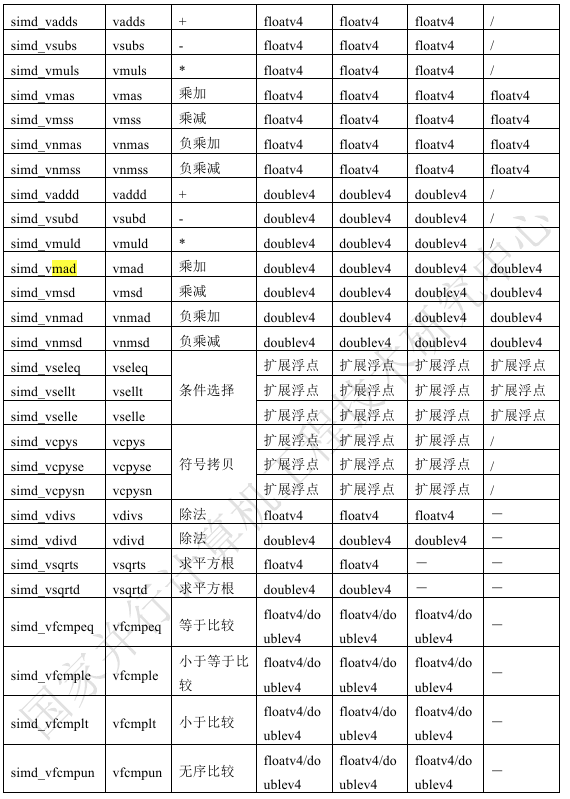
\includegraphics[width=12cm]{figure/sunway-simd.png}
  \end{center}

\subsubsection{Source code}
 We have compiled and executed the following source codes:

\verb`param.h`
\begin{code}
#define N 4096
#define I 64
#define Iv4 16

\end{code}

\verb`master.c`
\begin{code}
#include <stdlib.h>
#include <stdio.h>
#include <athread.h>
#include <sys/types.h>
#include <sys/stat.h>
#include <fcntl.h>

#include "param.h"

extern SLAVE_FUN(func)();

double a[N];
double b[N];
double c[N];

int main() {
  int i;
  printf("hello Sunway TaihuLight\n");

  for (i=0; i<N;++i){
    a[i] = i;
    b[i] = i;
  }

  // for (i=0; i<N;++i){
  //   c[i] = a[i] * b[i];
  // }
  athread_init();
  athread_spawn(func,0);//fflush(NULL);
  athread_join();

  for (i=1; i<N; i=2*i+1){
    printf("%d^2 == %lf\n", i, c[i]);
  }
  athread_halt();
  return 0;
}

\end{code}

\verb`slave.c`
\begin{code}
#include <slave.h>
#include <math.h>
#include <dma.h>

#include "param.h"

__thread_local volatile unsigned long get_reply, put_reply;
__thread_local doublev4 a_slave[Iv4], b_slave[Iv4], c_slave[Iv4];
extern double a[N], b[N], c[N];

void func() {
  int i;
  int my_id = athread_get_id(-1);
  int cid = my_id%8, rid = my_id/8;

  get_reply = 0;

  athread_get(PE_MODE, &a[my_id*I], &a_slave[0],I*8,&get_reply,0,0,0);
  athread_get(PE_MODE, &b[my_id*I], &b_slave[0],I*8,&get_reply,0,0,0);
  while(get_reply!=2) {}

  for(i=0;i<Iv4;i++){
    c_slave[i]=a_slave[i]*b_slave[i];
  }

  put_reply=0;
  athread_put(PE_MODE,&c_slave[0],&c[my_id * I],I*8,&put_reply,0,0);
  while(put_reply!=1) {}

}

\end{code}

\verb`run.sh`
\begin{code}

cd /home/export/base/nsccwuxi_riken/riken/online1/sandbox/nushio_box/sunway-test/03-slave-vector/src/
make && make run
    
\end{code}

\subsubsection{Results}

Got the following results:

\begin{code}
# 2017-02-14 13:05:28.457861
$ chmod 755 /home/nushio/hub/GB17/sunway-test/03-slave-vector/src/run.sh
$ ssh sunway 'mkdir -p /home/export/base/nsccwuxi_riken/riken/online1/sandbox/nushio_box/sunway-test/03-slave-vector/src/'
$ rsync -avz /home/nushio/hub/GB17/sunway-test/03-slave-vector/src/ sunway:/home/export/base/nsccwuxi_riken/riken/online1/sandbox/nushio_box/sunway-test/03-slave-vector/src/
sending incremental file list
./
Makefile
master.c
param.h
run.sh
slave.c

sent 1,385 bytes  received 117 bytes  429.14 bytes/sec
total size is 2,064  speedup is 1.37
$ ssh sunway /home/export/base/nsccwuxi_riken/riken/online1/sandbox/nushio_box/sunway-test/03-slave-vector/src//run.sh
sw5cc.new -O3 -msimd -host -E master.c > master.e
#	sw5cc.new -O3 -msimd -host -s master.c -o master.s
sw5cc.new -O3 -msimd -host -c master.c -o master.o
sw5cc.new -O3 -msimd -slave -E slave.c > slave.e
#sw5cc.new -O3 -msimd -slave -s slave.c -o slave.s
sw5cc.new -O3 -msimd -slave -c slave.c -o slave.o
sw5cc.new -hybrid  master.o slave.o -o main.out
bsub -I -b -q q_sw_expr -n 1 -cgsp 64 -share_size 4096 -host_stack 128 ./main.out
Job <6418407> has been submitted to queue <q_sw_expr>
some node is sleeping, waiting for dispatch ...
hello Sunway TaihuLight
1^2 == 1.000000
3^2 == 9.000000
7^2 == 49.000000
15^2 == 225.000000
31^2 == 961.000000
63^2 == 3969.000000
127^2 == 16129.000000
255^2 == 65025.000000
511^2 == 261121.000000
1023^2 == 1046529.000000
2047^2 == 4190209.000000
4095^2 == 16769025.000000
dispatching ...
Job 6418407 has been finished.

\end{code}

\subsubsection{Discussion}


We heve rewritten the previous example using
SIMD types and SIMD operations.


\subsection{Communicating between CPEs}
\subsubsection{Introduction}

CPEs form an 8x8 array, and
we can send the data in the row or the column direction in the CPE array.

The intrinsic functions
\verb`simd_putr` and
\verb`simd_putc` are used to send the data in the row nad the column direction, while
\verb`simd_getr` and
\verb`simd_getc` are used to recieve the data.

The second argument to the
\verb`simd_putr` and
\verb`simd_putc` functions
is the destination address. The address can be one of
(0...7) which specifies a column/row. The address can also be 8,
which means a broadcast.



\subsubsection{Source code}
 We have compiled and executed the following source codes:

\verb`param.h`
\begin{code}
#define N 256
#define I 4
#define Iv4 1

\end{code}

\verb`master.c`
\begin{code}
#include <stdlib.h>
#include <stdio.h>
#include <athread.h>
#include <sys/types.h>
#include <sys/stat.h>
#include <fcntl.h>

#include "param.h"

extern SLAVE_FUN(move_r)();
extern SLAVE_FUN(move_c)();

double a[N];
double b[N];
double c[N];

int main() {
  int i;
  athread_init();

  for (i=0; i<N;++i){
    a[i] = i/4;
    b[i] = i/4;
  }

  printf("before:");
  for (i=0; i<N; i++){
    if(i%4==0) printf(" ");
    if(i%32==0) printf("\n");
    printf("%2.0lf", a[i]);
  }
  printf("\n");

  athread_spawn(move_r,0);
  athread_join();

  printf("after move_r:");
  for (i=0; i<N; i++){
    if(i%4==0) printf(" ");
    if(i%32==0) printf("\n");
    printf("%2.0lf", c[i]);
  }
  printf("\n");

  athread_spawn(move_c,0);
  athread_join();

  printf("after move_c:");
  for (i=0; i<N; i++){
    if(i%4==0) printf(" ");
    if(i%32==0) printf("\n");
    printf("%2.0lf", c[i]);
  }
  printf("\n");

  athread_halt();
  return 0;
}

\end{code}

\verb`slave.c`
\begin{code}
#include <slave.h>
#include <math.h>
#include <dma.h>

#include "param.h"

__thread_local volatile unsigned long get_reply, put_reply;
__thread_local doublev4 a_slave[Iv4], b_slave[Iv4], c_slave[Iv4];
extern double a[N], b[N], c[N];

void move_r() {
  int i;
  int my_id = athread_get_id(-1);
  int cid = my_id%8, rid = my_id/8;

  get_reply = 0;

  athread_get(PE_MODE, &a[my_id*I], &a_slave[0],I*8,&get_reply,0,0,0);
  athread_get(PE_MODE, &b[my_id*I], &b_slave[0],I*8,&get_reply,0,0,0);
  while(get_reply!=2) {}

  simd_putr(a_slave[0], (cid+1)%8);
  c_slave[0] = simd_getr(c_slave[0]);

  put_reply=0;
  athread_put(PE_MODE,&c_slave[0],&c[my_id * I],I*8,&put_reply,0,0);
  while(put_reply!=1) {}

}

void move_c() {
  int i;
  int my_id = athread_get_id(-1);
  int cid = my_id%8, rid = my_id/8;

  get_reply = 0;

  athread_get(PE_MODE, &a[my_id*I], &a_slave[0],I*8,&get_reply,0,0,0);
  athread_get(PE_MODE, &b[my_id*I], &b_slave[0],I*8,&get_reply,0,0,0);
  while(get_reply!=2) {}

  simd_putc(b_slave[0], (rid*3)%8);
  c_slave[0] = simd_getc(c_slave[0]);

  put_reply=0;
  athread_put(PE_MODE,&c_slave[0],&c[my_id * I],I*8,&put_reply,0,0);
  while(put_reply!=1) {}

}

\end{code}

\verb`run.sh`
\begin{code}

cd /home/export/base/nsccwuxi_riken/riken/online1/sandbox/nushio_box/sunway-test/04-slave-comm/src/
make && make run
    
\end{code}

\subsubsection{Results}

Got the following results:

\begin{code}
# 2017-02-15 00:36:05.867609
$ chmod 755 /home/nushio/hub/GB17/sunway-test/04-slave-comm/src/run.sh
$ ssh sunway 'mkdir -p /home/export/base/nsccwuxi_riken/riken/online1/sandbox/nushio_box/sunway-test/04-slave-comm/src/'
$ rsync -avz /home/nushio/hub/GB17/sunway-test/04-slave-comm/src/ sunway:/home/export/base/nsccwuxi_riken/riken/online1/sandbox/nushio_box/sunway-test/04-slave-comm/src/
sending incremental file list
./
master.c
run.sh

sent 532 bytes  received 78 bytes  135.56 bytes/sec
total size is 2,906  speedup is 4.76
$ ssh sunway /home/export/base/nsccwuxi_riken/riken/online1/sandbox/nushio_box/sunway-test/04-slave-comm/src//run.sh
sw5cc.new -O3 -msimd -host -E master.c > master.e
#	sw5cc.new -O3 -msimd -host -s master.c -o master.s
sw5cc.new -O3 -msimd -host -c master.c -o master.o
sw5cc.new -hybrid  master.o slave.o -o main.out
bsub -I -b -q q_sw_expr -n 1 -cgsp 64 -share_size 4096 -host_stack 128 ./main.out
Job <6419585> has been submitted to queue <q_sw_expr>
waiting for dispatch ...
before: 
 0 0 0 0  1 1 1 1  2 2 2 2  3 3 3 3  4 4 4 4  5 5 5 5  6 6 6 6  7 7 7 7 
 8 8 8 8  9 9 9 9 10101010 11111111 12121212 13131313 14141414 15151515 
16161616 17171717 18181818 19191919 20202020 21212121 22222222 23232323 
24242424 25252525 26262626 27272727 28282828 29292929 30303030 31313131 
32323232 33333333 34343434 35353535 36363636 37373737 38383838 39393939 
40404040 41414141 42424242 43434343 44444444 45454545 46464646 47474747 
48484848 49494949 50505050 51515151 52525252 53535353 54545454 55555555 
56565656 57575757 58585858 59595959 60606060 61616161 62626262 63636363
after move_r: 
 7 7 7 7  0 0 0 0  1 1 1 1  2 2 2 2  3 3 3 3  4 4 4 4  5 5 5 5  6 6 6 6 
15151515  8 8 8 8  9 9 9 9 10101010 11111111 12121212 13131313 14141414 
23232323 16161616 17171717 18181818 19191919 20202020 21212121 22222222 
31313131 24242424 25252525 26262626 27272727 28282828 29292929 30303030 
39393939 32323232 33333333 34343434 35353535 36363636 37373737 38383838 
47474747 40404040 41414141 42424242 43434343 44444444 45454545 46464646 
55555555 48484848 49494949 50505050 51515151 52525252 53535353 54545454 
63636363 56565656 57575757 58585858 59595959 60606060 61616161 62626262
after move_c: 
 0 0 0 0  1 1 1 1  2 2 2 2  3 3 3 3  4 4 4 4  5 5 5 5  6 6 6 6  7 7 7 7 
24242424 25252525 26262626 27272727 28282828 29292929 30303030 31313131 
48484848 49494949 50505050 51515151 52525252 53535353 54545454 55555555 
 8 8 8 8  9 9 9 9 10101010 11111111 12121212 13131313 14141414 15151515 
32323232 33333333 34343434 35353535 36363636 37373737 38383838 39393939 
56565656 57575757 58585858 59595959 60606060 61616161 62626262 63636363 
16161616 17171717 18181818 19191919 20202020 21212121 22222222 23232323 
40404040 41414141 42424242 43434343 44444444 45454545 46464646 47474747
dispatching ...
Job 6419585 has been finished.

\end{code}

\subsubsection{Discussion}

We have confirmed that
\verb`simd_putr` sends the data in the row direction, and
\verb`simd_putc` sends the data in the column direction.


\subsection{SIMD arithmetic instructions (TODO)}
\subsubsection{Introduction}

We need to use the SIMD intrinsics of Sunway TaihuLight to make use of its full computing potential.
The SIMD intrinsic expressions accept SIMD types such as
\verb`intv8`,
\verb`doublev4`,
\verb`floatv4`.


We will test the effects of the SIMD intrinsics.


\subsubsection{Source code}
 We have compiled and executed the following source codes:

\verb`param.h`
\begin{code}
#define N 4096
#define I 64
#define Iv4 16

\end{code}

\verb`master.c`
\begin{code}
#include <stdlib.h>
#include <stdio.h>
#include <athread.h>
#include <sys/types.h>
#include <sys/stat.h>
#include <fcntl.h>

#include "param.h"

extern SLAVE_FUN(func)();

double a[N];
double b[N];
double c[N];

int main() {
  int i;
  printf("hello Sunway TaihuLight\n");

  for (i=0; i<N;++i){
    a[i] = i;
    b[i] = i;
  }

  // for (i=0; i<N;++i){
  //   c[i] = a[i] * b[i];
  // }
  athread_init();
  athread_spawn(func,0);//fflush(NULL);
  athread_join();

  for (i=1; i<N; i=2*i+1){
    printf("%d^2 == %lf\n", i, c[i]);
  }
  athread_halt();
  return 0;
}

\end{code}

\verb`slave.c`
\begin{code}
#include <slave.h>
#include <math.h>
#include <dma.h>

#include "param.h"

__thread_local volatile unsigned long get_reply, put_reply;
__thread_local doublev4 a_slave[Iv4], b_slave[Iv4], c_slave[Iv4];
extern double a[N], b[N], c[N];

void func() {
  int i;
  int my_id = athread_get_id(-1);
  int cid = my_id%8, rid = my_id/8;

  get_reply = 0;

  athread_get(PE_MODE, &a[my_id*I], &a_slave[0],I*8,&get_reply,0,0,0);
  athread_get(PE_MODE, &b[my_id*I], &b_slave[0],I*8,&get_reply,0,0,0);
  while(get_reply!=2) {}

  for(i=0;i<Iv4;i++){
    c_slave[i]=a_slave[i]*b_slave[i];
  }

  put_reply=0;
  athread_put(PE_MODE,&c_slave[0],&c[my_id * I],I*8,&put_reply,0,0);
  while(put_reply!=1) {}

}

\end{code}

\verb`run.sh`
\begin{code}

cd /home/export/base/nsccwuxi_riken/riken/online1/sandbox/nushio_box/sunway-test/05-slave-sqrt/src/
make && make run
    
\end{code}

\subsubsection{Results}

Got the following results:

\begin{code}
# 2017-02-15 13:46:19.548559
$ chmod 755 /home/nushio/hub/FDPS/sandbox/nushio_box/sunway-test/05-slave-sqrt/src/run.sh
$ ssh sunway 'mkdir -p /home/export/base/nsccwuxi_riken/riken/online1/sandbox/nushio_box/sunway-test/05-slave-sqrt/src/'
$ rsync -avz /home/nushio/hub/FDPS/sandbox/nushio_box/sunway-test/05-slave-sqrt/src/ sunway:/home/export/base/nsccwuxi_riken/riken/online1/sandbox/nushio_box/sunway-test/05-slave-sqrt/src/
sending incremental file list
run.sh

sent 173 bytes  received 40 bytes  28.40 bytes/sec
total size is 2,062  speedup is 9.68
$ ssh sunway /home/export/base/nsccwuxi_riken/riken/online1/sandbox/nushio_box/sunway-test/05-slave-sqrt/src//run.sh
sw5cc.new -O3 -msimd -host -E master.c > master.e
#	sw5cc.new -O3 -msimd -host -s master.c -o master.s
sw5cc.new -O3 -msimd -host -c master.c -o master.o
sw5cc.new -O3 -msimd -slave -E slave.c > slave.e
#sw5cc.new -O3 -msimd -slave -s slave.c -o slave.s
sw5cc.new -O3 -msimd -slave -c slave.c -o slave.o
sw5cc.new -hybrid  master.o slave.o -o main.out
bsub -I -b -q q_sw_expr -n 1 -cgsp 64 -share_size 4096 -host_stack 128 ./main.out
Job <6420164> has been submitted to queue <q_sw_expr>
waiting for dispatch ...
hello Sunway TaihuLight
1^2 == 1.000000
3^2 == 9.000000
7^2 == 49.000000
15^2 == 225.000000
31^2 == 961.000000
63^2 == 3969.000000
127^2 == 16129.000000
255^2 == 65025.000000
511^2 == 261121.000000
1023^2 == 1046529.000000
2047^2 == 4190209.000000
4095^2 == 16769025.000000
dispatching ...
Job 6420164 has been finished.

\end{code}

\subsubsection{Discussion}

TODO


\subsection{Using the C++ compiler}
\subsubsection{Introduction}

You can use C++ compiler in TaihuLight.



\subsubsection{Source code}
 We have compiled and executed the following source codes:

\verb`master.cpp`
\begin{code}
#include <stdlib.h>
#include <stdio.h>
#include <athread.h>
#include <sys/types.h>
#include <sys/stat.h>
#include <fcntl.h>

#define N 4096


extern SLAVE_FUN(func)();

double a[N];
double b[N];
double c[N];

int main() {
  int i;
  printf("hello Sunway TaihuLight\n");

  for (i=0; i<N;++i){
    a[i] = i;
    b[i] = i;
  }

  // for (i=0; i<N;++i){
  //   c[i] = a[i] * b[i];
  // }
  athread_init();
  athread_spawn(func,0);//fflush(NULL);
  athread_join();

  for (i=1; i<N; i=2*i+1){
    printf("%d^2 == %lf\n", i, c[i]);
  }
  athread_halt();
  return 0;
}

\end{code}

\verb`slave.c`
\begin{code}
#include <slave.h>
#include <math.h>
#include <dma.h>

#define N 4096
#define I 64

__thread_local volatile unsigned long get_reply, put_reply;
__thread_local int my_id;
__thread_local double a_slave[I], b_slave[I], c_slave[I];
extern double a[N], b[N], c[N];

void func() {
  int i;
  my_id = athread_get_id(-1);
  get_reply = 0;

  athread_get(PE_MODE, &a[my_id*I], &a_slave[0],I*8,&get_reply,0,0,0);
  athread_get(PE_MODE, &b[my_id*I], &b_slave[0],I*8,&get_reply,0,0,0);
  while(get_reply!=2) {}

  for(i=0;i<I;i++){
    c_slave[i]=a_slave[i]*b_slave[i];
  }

  put_reply=0;
  athread_put(PE_MODE,&c_slave[0],&c[my_id * I],I*8,&put_reply,0,0);
  while(put_reply!=1) {}

}

\end{code}

\verb`run.sh`
\begin{code}

cd /home/export/base/nsccwuxi_riken/riken/online1/sandbox/nushio_box/sunway-test/02-slave/src/
make && make run
    
\end{code}

\subsubsection{Results}

Got the following results:

\begin{code}
TODO

\end{code}

\subsubsection{Discussion}

TODO




\section{Practical Applications} \label{sec:practical}

\subsection{Introduction to the practical application section}

% 実践編では、Sunway TaihuLightである程度まとまったプログラムを作って
% いく。具体的には、村主の担当分野であるTemporal Blockingをかけたステ
% ンシルアプリケーションを主に作りながら、TaihuLightでどうすれば性能が
% 出るかを検証していく。

In \S \ref{sec:practical}, we create larger programs

\subsection{1CG (Core Group)でのTemporal Blocking実験}
\subsubsection{Introduction}

Sunway での研究開発の方針として、まずは簡単な差分ステンシルを用い、1CGで
temporal blocking で性能を出すことがそもそも可能かどうかを確認してみることにする。

ここでの「性能を出す」とは、ローカルメモリサイズ、主記憶バンド幅から理論的に可能な性能に比べて
何\%の演算性能が実現可能かを確認するということである。


この実験は1プロセスで行うので並列化とか通信は考えないでやることができて、実際、少し
規模が大きい問題を考えるとノード間通信の時間はほぼ無視できるので通信と
計算を無理にオーバーラップさせる必要はなくなる。もっとも
定量的、実験的にちゃんと見積もっておく必要はある。



この実験で駄目なら何やっても駄目だし、これでできるなら基本には同じやり方で
コード生成できれば色々他のことができることになる。


\subsubsection{理論的に実現可能な演算性能の見積もり}

理論的に実現可能な演算性能は以下のように見積もられる。

演算器の演算性能および主記憶の帯域幅を
$F$ Flop/s および
$B$ Byte/s とする。またステンシル計算の1メッシュあたりの演算量および、独立変数の情報量を
$C$ Flop, $H$ Byte とする。

すると、Spatial Blockingをもちいる場合、1秒間に更新可能なメッシュ数
$n_{up}$は、

\begin{align}
n_{up} &= \min \left( \frac{B}{2H}, \frac{F}{C} \right)
\end{align}

で見積もられる。そして、実効性能は

\begin{align}
  F_{up} &= C \cdot n_{up} \\
  &= \min \left( \frac{BC}{2H}, F \right)
\end{align}

で見積もられる。


Temporal Blockingをもちいる場合、1秒間に更新可能なメッシュ数
$n_{up}$は、キャッシュに当てたタイルサイズを$N_T$、
空間の次元を$d$、
ステンシルの袖領域のサイズを$N_s$として

\begin{align}
n_{up} &= \min \left( \frac{N_T B}{4dN_s H}, \frac{F}{C} \right)
\end{align}

で見積もられる。そして、実効性能は

\begin{align}
  F_{up} &= C \cdot n_{up} \\
  &= \min \left( \frac{N_T B C}{4 d N_s H}, F \right)
\end{align}

で見積もられる。




\subsubsection{Source code}
 We have compiled and executed the following source codes:

\verb`param.h`
\begin{code}
#define NX 50
#define NY 50
#define NZ 50

#define SX 34
#define SY 34
#define SZ 34

#define T_MAX 3000

typedef double Real;


const Real Fu = 1.0/86400, Fv = 6.0/86400, Fe = 1.0/900, Du = 0.1*2.3e-9, Dv = 12.2e-11;
const Real dt = 0*200, dx = 0.001;

\end{code}

\verb`master.c`
\begin{code}
#include <stdio.h>
#include <athread.h>
#include <fcntl.h>
#define N 4096


//extern SLAVE_FUN(func)();

double a[N];
double b[N];
double c[N];

int main() {
  int i;
  printf("hello Sunway TaihuLight\n");

  for (i=0; i<N;++i){
    a[i] = i;
    b[i] = i;
  }

  for (i=0; i<N;++i){
    c[i] = a[i] * b[i];
  }

  for (i=1; i<N; i=2*i+1){
    printf("%d^2 == %lf\n", i, c[i]);
  }

  return 0;
}

\end{code}

\verb`master.cpp`
\begin{code}
#include <cmath>
#include <unistd.h>
#include <fstream>
#include <iostream>
#include <sstream>
#include <sys/time.h>

#include "param.h"



Real U[NX][NY][NZ], V[NX][NY][NZ];
Real U_other[NX][NY][NZ], V_other[NX][NY][NZ];
int global_clock;


Real Uwx[T_MAX][2][SY][SZ], Uwy[T_MAX][SX][2][SZ], Uwz[T_MAX][SX][SY][2];
Real Vwx[T_MAX][2][SY][SZ], Vwy[T_MAX][SX][2][SZ], Vwz[T_MAX][SX][SY][2];

Real sU0[SX][SY][SZ], sV0[SX][SY][SZ];


extern "C" {
  void run_benchmark();
}

double wctime() {
  struct timeval tv;
  gettimeofday(&tv,NULL);
  return (double)tv.tv_sec + (double)tv.tv_usec*1e-6;
}



void fill_initial_condition() {
  global_clock=0;
  for (int x=0;x<NX;++x) {
    for (int y=0;y<NY;++y) {
      for (int z=0;z<NZ;++z) {
        U[x][y][z] = 1;
        V[x][y][z] = 0;
      }
    }
  }
  int bx = std::max(NX/4,NX/2-8),  ex = std::min(3*NX/4+1,NX/2+8);
  int by = std::max(NY/4,NY/2-8),  ey = std::min(3*NY/4+1,NY/2+8);
  int bz = std::max(NZ/4,NZ/2-8),  ez = std::min(3*NZ/4+1,NZ/2+8);
  for (int x=bx;x<ex;++x){
    for (int y=by;y<ey;++y){
      for (int z=bz;z<ez;++z){
        U[x][y][z] = 0.5;
        V[x][y][z] = 0.25+0.1*sin(x+sqrt(y)+cos(z));
      }
    }
  }
}


inline Real periodic(Real ar[NX][NY][NZ],int x, int y, int z) {
  x = ((x+100*NX)%NX+NX)%NX;
  y = ((y+100*NY)%NY+NY)%NY;
  z = ((z+100*NZ)%NZ+NZ)%NZ;
  //x = (x+NX)%NX;
  //y = (y+NY)%NY;
  //z = (z+NZ)%NZ;
  return ar[x][y][z];
}


void naive_proceed() {
  ++global_clock;

  auto lap = [](Real ar[NX][NY][NZ],int x, int y, int z) {
    auto ret = periodic(ar, x-1, y, z) + periodic(ar, x+1, y, z)
    + periodic(ar, x, y-1, z) + periodic(ar, x, y+1, z)
    + periodic(ar, x, y, z-1) + periodic(ar, x, y, z+1)
    - 6*ar[x][y][z];
    return ret / dx / dx;
  };

  for (int x=0;x<NX;++x) {
    for (int y=0;y<NY;++y) {
      for (int z=0;z<NZ;++z) {
        auto u = U[x][y][z],  v = V[x][y][z];
        auto du_dt = -Fe * u*v*v + Fu*(1-u) + Du * lap(U,x,y,z);
        auto dv_dt =  Fe * u*v*v - Fv*v     + Dv * lap(V,x,y,z);
        U_other[x][y][z] = U[x][y][z] + dt*du_dt;
        V_other[x][y][z] = V[x][y][z] + dt*dv_dt;
      }
    }
  }

  for (int x=0;x<NX;++x) {
    for (int y=0;y<NY;++y) {
      for (int z=0;z<NZ;++z) {
        U[x][y][z]=U_other[x][y][z];
      }
    }
  }
  for (int x=0;x<NX;++x) {
    for (int y=0;y<NY;++y) {
      for (int z=0;z<NZ;++z) {
        V[x][y][z]=V_other[x][y][z];
      }
    }
  }
}

void get_solution_at(int t, int x, int y, int z, Real &u, Real &v) {
  if(global_clock > t) fill_initial_condition();
  while(global_clock < t) naive_proceed();
  u = periodic(U,x,y,z);
  v = periodic(V,x,y,z);
}

int main () {

  fill_initial_condition();
  for(int x=0;x<SX;++x) {
    for(int y=0;y<SY;++y) {
      for(int z=0;z<SZ;++z) {
        double u,v; get_solution_at(0,x,y,z, u,v);
        sU0[x][y][z]=u;
        sV0[x][y][z]=v;
      }
    }
  }

  std::cerr << "Setting up wall values..." << std::endl;
  for(int t = 0;t<T_MAX;++t){
    for(int x=SX-2;x<SX;++x) {
      for(int y=0;y<SY;++y) {
        for(int z=0;z<SZ;++z) {
          double u,v; get_solution_at(t,x+t,y+t,z+t, u,v);
          Uwx[t][x-(SX-2)][y][z] = u;
          Vwx[t][x-(SX-2)][y][z] = v;
        }
      }
    }

    for(int x=0;x<SX;++x) {
      for(int y=SY-2;y<SY;++y) {
        for(int z=0;z<SZ;++z) {
          double u,v; get_solution_at(t,x+t,y+t,z+t, u,v);
          Uwy[t][x][y-(SY-2)][z] = u;
          Vwy[t][x][y-(SY-2)][z] = v;
        }
      }
    }

    for(int x=0;x<SX;++x) {
      for(int y=0;y<SY;++y) {
        for(int z=SZ-2;z<SZ;++z) {
          double u,v; get_solution_at(t,x+t,y+t,z+t, u,v);
          Uwz[t][x][y][z-(SZ-2)] = u;
          Vwz[t][x][y][z-(SZ-2)] = v;
        }
      }
    }
  }


  for(int trial=0;trial<10;++trial) {

    double time_begin = wctime();

    run_benchmark();

    double time_end = wctime();

    double flop = 29.0 * (SX-2)*(SY-2)*(SZ-2) *T_MAX;
    double time_elapse = time_end-time_begin;

    {
      const int t = T_MAX;
      double num=0,den=0;
      for(int x=0;x<SX-2;++x) {
        for(int y=0;y<SY-2;++y) {
          for(int z=0;z<SZ-2;++z) {
            double u,v; get_solution_at(t,x+t,y+t,z+t, u,v);
            num += std::abs(u-sU0[x][y][z]);
            den += 1;
          }
        }
      }
      std::ostringstream msg;
      msg << SX << " " << SY << " " << SZ << " " << T_MAX << " "
          << " t: " << time_elapse << " GFlops: " << flop/time_elapse/1e9<< " error: " << (num/den);
      std::ofstream log_file("benchmark.txt", std::ios::app);
      std::cout << msg.str() << std::endl;
      log_file << msg.str() << std::endl;
    }
  }
}

\end{code}

\verb`slave.c`
\begin{code}
#include <stdio.h>
#include "param.h"

extern Real sU0[SX][SY][SZ], sV0[SX][SY][SZ];
extern Real Uwx[T_MAX][2][SY][SZ], Uwy[T_MAX][SX][2][SZ], Uwz[T_MAX][SX][SY][2];
extern Real Vwx[T_MAX][2][SY][SZ], Vwy[T_MAX][SX][2][SZ], Vwz[T_MAX][SX][SY][2];


// double-buffered simulation state
Real sU[SX][SY][SZ], sV[SX][SY][SZ];
Real sU_1[SX][SY][SZ], sV_1[SX][SY][SZ];


void run_benchmark(){

  printf("Carrying out simulation...\n");

  // set initial condition
  for(int x=0;x<SX;++x) {
    for(int y=0;y<SY;++y) {
      for(int z=0;z<SZ;++z) {
        sU[x][y][z]=sU0[x][y][z];
        sV[x][y][z]=sV0[x][y][z];
      }
    }
  }

  for(int t = 0; t < T_MAX; ++t){
    // load communication values
    for(int x=SX-2;x<SX;++x) {
      for(int y=0;y<SY;++y) {
        for(int z=0;z<SZ;++z) {
          sU[x][y][z] = Uwx[t][x-(SX-2)][y][z];
          sV[x][y][z] = Vwx[t][x-(SX-2)][y][z];
        }
      }
    }

    for(int x=0;x<SX-2;++x) {
      for(int y=SY-2;y<SY;++y) {
        for(int z=0;z<SZ;++z) {
          sU[x][y][z] = Uwy[t][x][y-(SY-2)][z];
          sV[x][y][z] = Vwy[t][x][y-(SY-2)][z];
        }
      }
    }

    for(int x=0;x<SX-2;++x) {
      for(int y=0;y<SY-2;++y) {
        for(int z=SZ-2;z<SZ;++z) {
          sU[x][y][z] = Uwz[t][x][y][z-(SZ-2)];
          sV[x][y][z] = Vwz[t][x][y][z-(SZ-2)];
        }
      }
    }



    // destructively update the state
#define lap(ar, x, y, z)                        \
    ( ar[x][y+1][z+1] + ar[x+2][y+1][z+1]       \
      + ar[x+1][y][z+1] + ar[x+1][y+2][z+1]     \
      + ar[x+1][y+1][z] + ar[x+1][y+1][z+2]     \
        - 6*ar[x+1][y+1][z+1]) / dx / dx

    for(int x=0;x<SX-2;++x) {
      for(int y=0;y<SY-2;++y) {
        for(int z=0;z<SZ-2;++z) {
          Real u=sU[x+1][y+1][z+1] ;
          Real v=sV[x+1][y+1][z+1] ;

          Real du_dt = -Fe * u*v*v + Fu*(1-u) + Du * lap(sU,x,y,z);
          Real dv_dt =  Fe * u*v*v - Fv*v     + Dv * lap(sV,x,y,z);
          sU_1[x][y][z] = u+dt*du_dt;
          sV_1[x][y][z] = v+dt*dv_dt;
        }
      }
    }


    for(int x=0;x<SX-2;++x) {
      for(int y=0;y<SY-2;++y) {
        for(int z=0;z<SZ-2;++z) {
          sU[x][y][z] = sU_1[x][y][z];
          sV[x][y][z] = sV_1[x][y][z];
        }
      }
    }
  }

  // return the final condition
  for(int x=0;x<SX;++x) {
    for(int y=0;y<SY;++y) {
      for(int z=0;z<SZ;++z) {
        sU0[x][y][z]=sU[x][y][z];
        sV0[x][y][z]=sV[x][y][z];
      }
    }
  }

}

\end{code}

\verb`run.sh`
\begin{code}

cd /home/export/base/nsccwuxi_riken/riken/online1/sandbox/nushio_box/sunway-test/01-master/src/
make && make run
    
\end{code}

\subsubsection{Results}

Got the following results:

\begin{code}
TODO

\end{code}

\subsubsection{Discussion}


理論的に実現可能な性能の性能のTODO\%の性能を得た。




\end{document}
